\documentclass[twocolumn,a4j]{jsarticle}
\setlength{\topmargin}{-18.5cm}
\setlength{\oddsidemargin}{-8.5mm}
\setlength{\evensidemargin}{-8.5mm}
\setlength{\textwidth}{19cm}
\setlength{\textheight}{26.5cm}

\usepackage[top=15truemm,bottom=20truemm,left=20truemm,right=20truemm]{geometry}
\usepackage[latin1]{inputenc}
\usepackage{amsmath}
\usepackage{amsfonts}
\usepackage{amssymb}
\usepackage[dvipdfmx]{graphicx}
\usepackage[hang,small,bf]{caption}
\usepackage[subrefformat=parens]{subcaption}
\usepackage[dvipdfmx]{color}
\usepackage{listings}
\usepackage{listings,jvlisting}
\usepackage{geometry}
\usepackage{framed}
\usepackage{color}
\usepackage[dvipdfmx]{hyperref}
\usepackage{ascmac}
\usepackage{enumerate}
\usepackage{tabularx}
\usepackage{cancel}
\usepackage{scalefnt}
\usepackage{overcite}
\usepackage{otf}
\usepackage{multicol}
\usepackage[geometry]{ifsym}

\renewcommand{\figurename}{Fig.}
\renewcommand{\tablename}{Table }

\hypersetup{%
    hidelinks %リンクの色消し
}

\lstset{
basicstyle={\ttfamily},
identifierstyle={\small},
commentstyle={\smallitshape},
keywordstyle={\small\bfseries},
ndkeywordstyle={\small},
stringstyle={\small\ttfamily},
frame={tb},
breaklines=true,
columns=[l]{fullflexible},
xrightmargin=0zw,
xleftmargin=3zw,
numberstyle={\scriptsize},
stepnumber=1,
numbersep=1zw,
lineskip=-0.5ex
}

% キャプション後ろのダブルコロンを消す
\makeatletter
\long\def\@makecaption#1#2{%
  \vskip\abovecaptionskip
  \iftdir\sbox\@tempboxa{#1\hskip1zw#2}%
    \else\sbox\@tempboxa{#1 #2}%
  \fi
  \ifdim \wd\@tempboxa >\hsize
    \iftdir #1\hskip1zw#2\relax\par
      \else #1 #2\relax\par\fi
  \else
    \global \@minipagefalse
    \hbox to\hsize{\hfil\box\@tempboxa\hfil}%
  \fi
  \vskip\belowcaptionskip}
\makeatother


\makeatletter
\def\@maketitle
{
\begin{center}
{\LARGE \@title \par}
\end{center}
\begin{flushright}
{\large \@date}\\
{\large 京都工芸繊維大学 大学院 機械設計学専攻 計測システム工学研究室}\\
{\large M2 \@author}
\end{flushright}
\par\vskip 1.5em
}
\makeatother

\author{来代 勝胤 / KITADAI Masatsugu}
\title{令和5年度 11月度 月例報告書}
\date{2023/12/05}

\begin{document}
\columnseprule=0.1mm
\maketitle

\section*{報告内容}
\begin{enumerate}[1.]
  \item [0.] 修士論文について
  \item 序論
  \item 粒子クラスタを用いた粒子追跡アルゴリズム
  \item 12月の予定
\end{enumerate}

\setcounter{section}{-1}
\section{修士論文について}

\begin{table}[hbtp]
  \section*{$\blacksquare$ 題目}
  \centering
  \begin{tabular}{c}
    \hline
    多重カラーLLSを用いた二次流れPIV計測法  \\ \hline
    PIV Mesurement Method of Secondary Flow \\
    Using Multi-Color LLS                   \\ \hline
  \end{tabular}
\end{table}

\begin{table}[hbtp]
  \centering
  \section*{$\blacksquare$ 構成}
  \begin{tabular}{r c l}
    \hline
    1. & \gt{序論}     & \begin{tabular}{l} 二次流れ計測の重要性と\\計測手法の課題 \end{tabular}            \\ \hline
    2. & \gt{計測手法} & \begin{tabular}{l} 粒子クラスタを用いた\\粒子追跡アルゴリズム \end{tabular}        \\ \hline
    3. & \gt{数値解析} & \begin{tabular}{l} 数値解析を用いた\\アルゴリズムの性能評価   \end{tabular}        \\ \hline
    4. & \gt{基礎実験} & \begin{tabular}{l} 三角翼後流の計測結果\\ (比較的安定した流れの計測 \end{tabular} \\ \hline
    5. & \gt{応用実験} & \begin{tabular}{l} 車両モデル後流の計測結果\\ (不安定な流れの計測) \end{tabular} \\ \hline
    6. & \gt{結論}                                                                                          \\ \hline
  \end{tabular}
\end{table}

\section{序論}
輸送機械の設計および開発を行う際,流体による作用力の影響を考慮しなければならない.
特に進行を妨げる方向にはたらく抗力の低減は,輸送機械の燃費向上を考える上で非常に重要だといえる.
また,輸送機械の設計・開発において抗力を考慮する際には,
機体周りの流れ場および主流方向に垂直な面内の二次流れ構造の理解が必要不可欠である.
ここで,流体計測手法においては,レーザー光をシート状に拡散し,
その平面内を通過するトレーサー粒子を撮影することで流れ場を得る
Particle Image Velocimetry (PIV) を用いた計測手法がある.
特にPIVでは,対象の流れ場を,移動量ベクトルを用いて定量的に評価することが可能であるが,
一般的に主流方向を面内に含めて計測を行うことが多く,二次流れを対象とした計測例は少ない.
そこで,Laser Light Sheet (LLS) を用いた二次流れの時系列解析手法を提案し,性能評価を行ってきた.
本研究では,この手法を用いて三角翼および車両モデル後方に発生する
二次流れのPIV計測を行い,実用性を検証した.

\section{計測手法}
\begin{figure}[htbp]
  \centering
  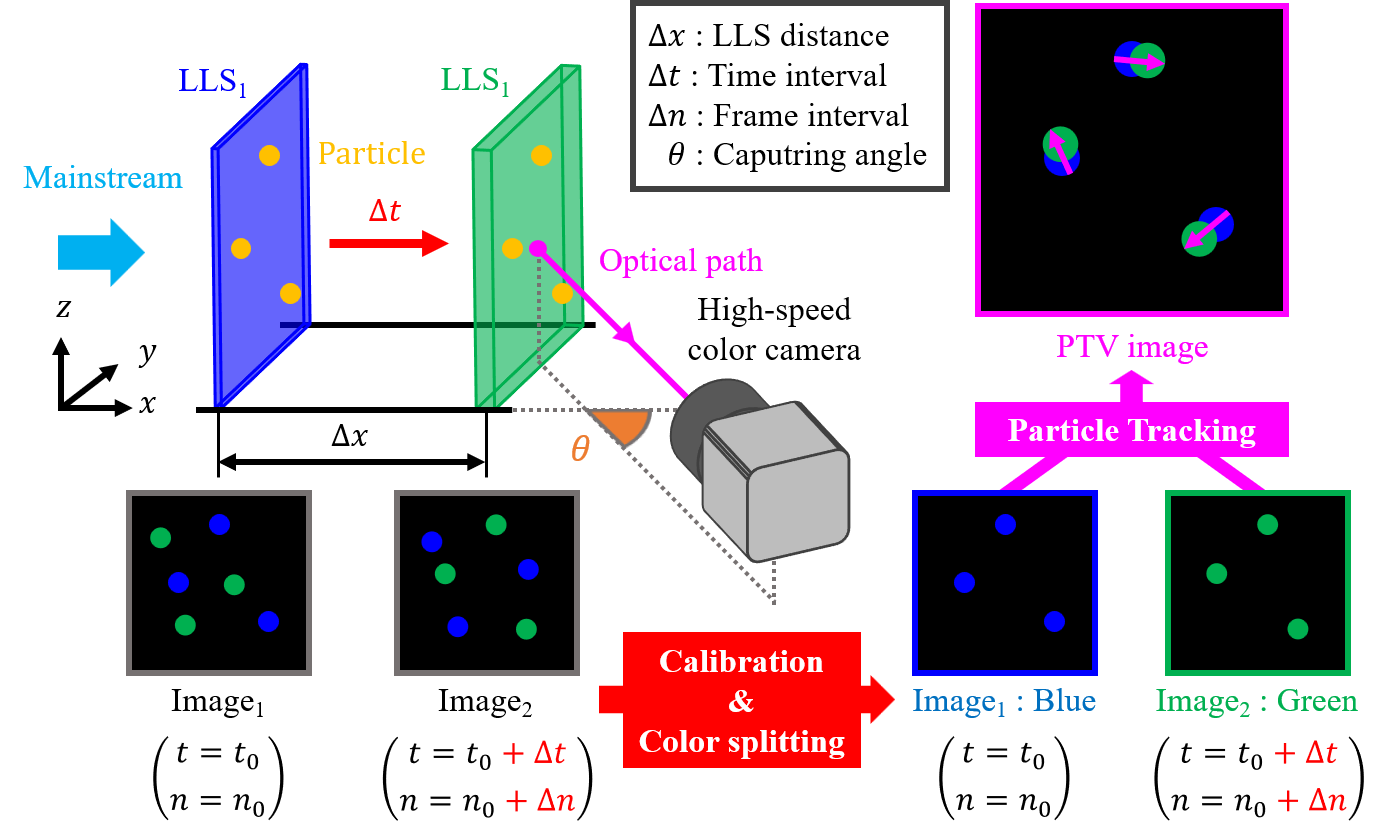
\includegraphics[keepaspectratio, width=80mm]{../images/PIVMethodforSecondaryFlow.png}
  \caption{PIV method for secondary flow analysis}
\end{figure}

主流方向に対して垂直に異なる2色のLLSを,間隔$\Delta x$をもって設置する.
それらを通過する粒子像を取得し,画像解析を行うことで二次流れの速度場を得る
このとき,$\rm{LLS}_1$を時刻 $t_0$ に通過するときに撮影される粒子像を$\rm{Image}_2$とし,
$n_0$ 枚目の画像とする.その後,同一の粒子群は$\Delta t$秒後に$\Delta x$だけ
下流側の$\rm{LLS}_2$に到達すると考えられ,
通過する時刻$t_0 + \Delta t$に撮影される粒子像を$\rm{Image}_2$としたとき,
$n_0 + \Delta n$枚目の画像となる.
ここで,$n_0$枚目に示される$\rm{LLS}_1$の粒子像と$n_0 + \Delta n$枚目に示される
$\rm{LLS}_2$の粒子像について,PTV (Particle Tracking Velocimetry) を適用することで,
主流方向に垂直な面内の速度場の速度場を得ることができる.

\setcounter{section}{3}
\section{基礎実験}
\subsection{実験装置}
本研究では,Fig.1 で示したシステムを Fig.2 に示す光学系と回流水槽を用いて構成する.
LLSについて,上流側に488 nm(青:B),下流側に532 nm (緑:G)を使用した.
また,モデル後方からの撮影は不可能であることから,
アクリル製の水槽を使用して屈折の影響を排除し,
モデル斜め後方から撮影している.\\

\begin{figure}[htbp]
  \centering
  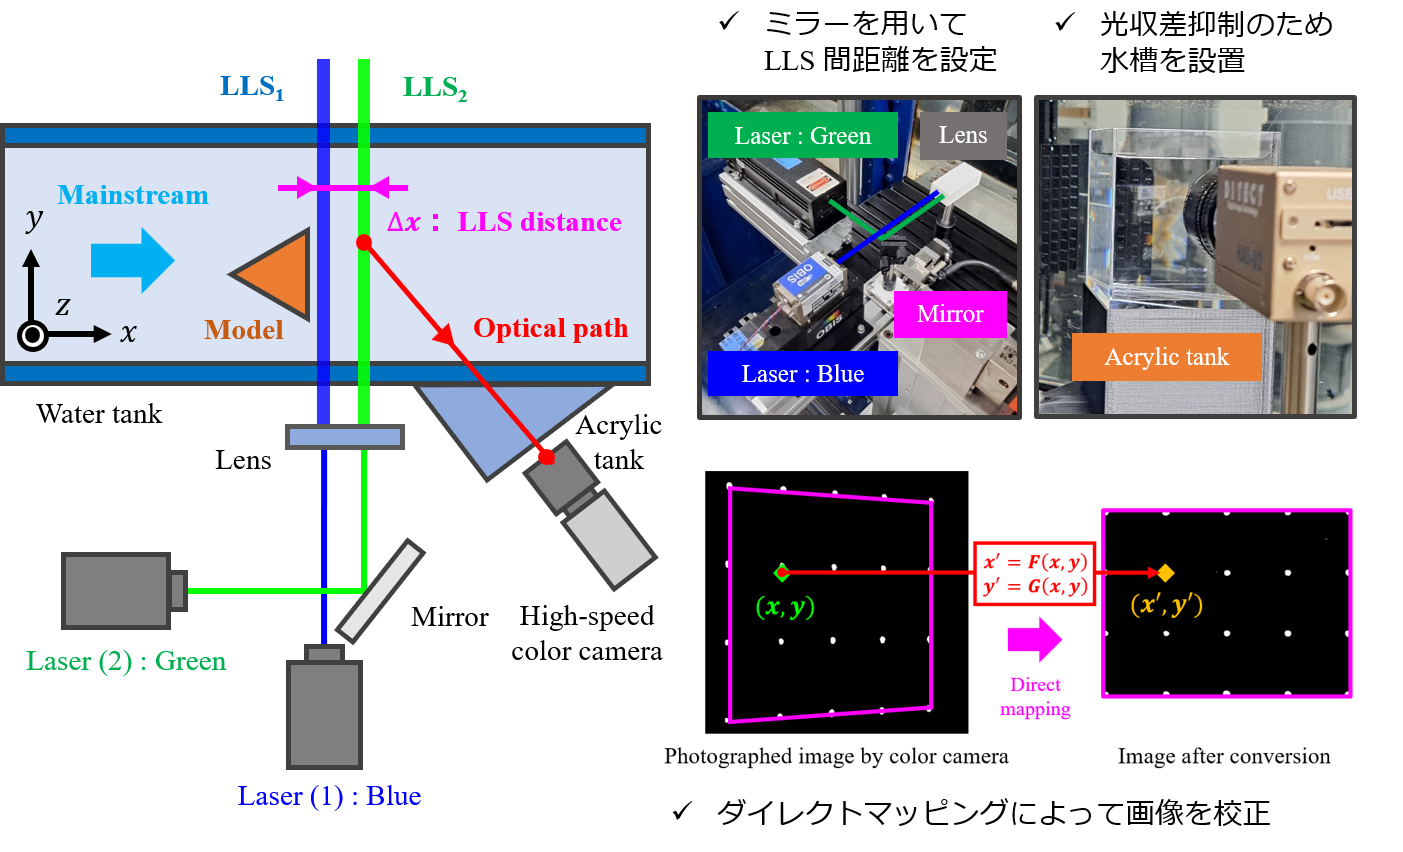
\includegraphics[keepaspectratio, width=80mm]{../images/ExperimentalLayout.png}
  \caption{Experimental layout}
\end{figure}

\subsection{三角翼後流の計測}
本手法の実用性を確かめるため,Fig.3 に示す一辺が
120 mm の正三角形状の三角翼モデルを用いて基礎性能評価実験を行った.
モデル後端から 50 mm の位置を対象とし,二次流れの計測を行う.
また,代表長さを三角翼における翼幅 120 mm,
水の動粘性係数を標準状態における 1.000 $\rm{mm}^2/\rm{s}$,
主流方向速度を 250 $\rm{mm}/\rm{s}$とすると,
レイノルズ数Reは以下のように計算される.
\begin{eqnarray*}
  \rm{Re} = \frac{250 \times 120}{1.000} = 3.0 \times 10^4
\end{eqnarray*}

\begin{figure}[htbp]
  \centering
  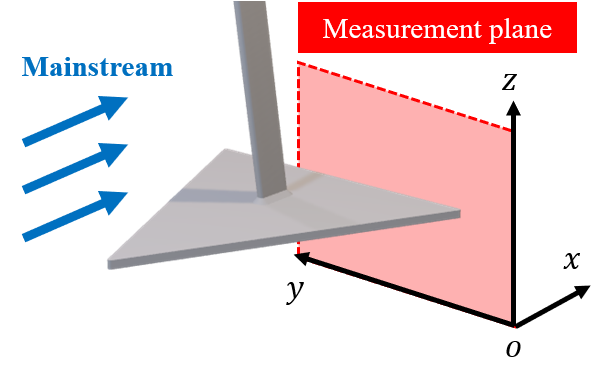
\includegraphics[keepaspectratio, width=60mm]{../images/ImageofDeltaWing.png}
  \caption{Delta wing model}
\end{figure}

\subsection{計測結果}
Fig.5 に 2mm 間隔の格子点上に速度ベクトルを再配置した時間平均の結果を示す.
結果をみると翼端を中心に反時計回りの渦が発生していることがわかる.
(a) のカラーマップは渦度を示しており,$y-z$平面内のベクトルの示す反時計回りの渦中心に
強い渦度を持つことがわかる.また,その右隣に小さな時計回り(負)の渦を持つことがわかる.
また,粒子クラスタの情報を用いて主流方向速度を推定すると,
それぞれの渦中心において主流方向速度が小さくなっていることがわかる.

\begin{figure}[htbp]
  \centering
  {
    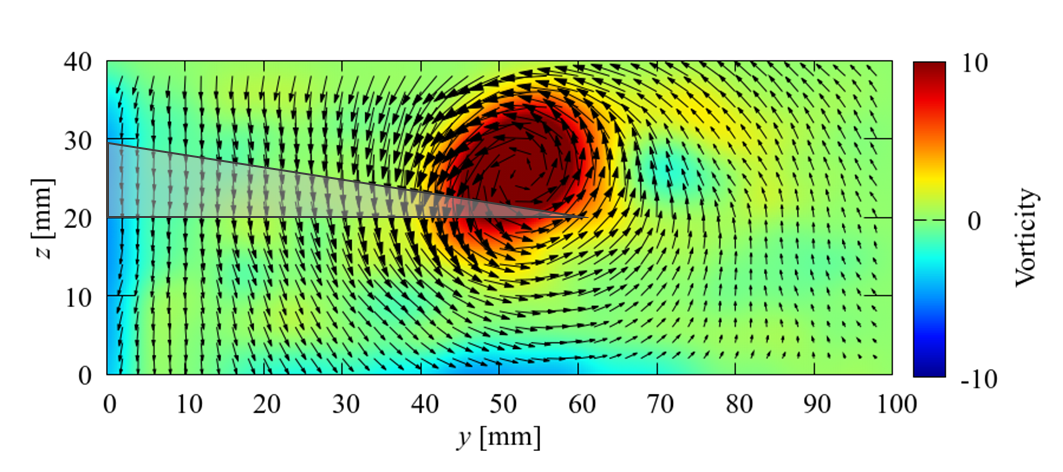
\includegraphics[keepaspectratio, width=85mm]{../images/WakeofDeltaWing_Vorticity_x=50.png}
    \subcaption{Velocity $(v, w)$ and Vorticity}
    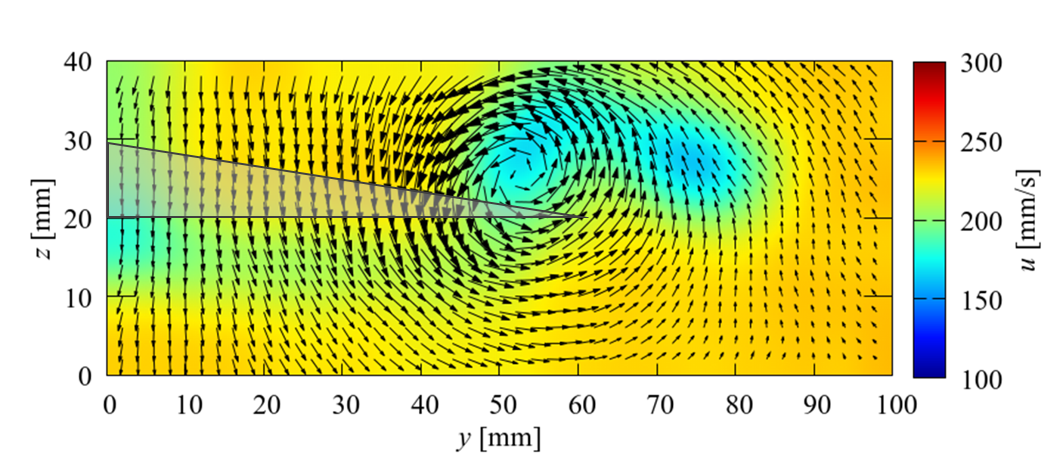
\includegraphics[keepaspectratio, width=85mm]{../images/WakeofDeltaWing_Velocity_x=50.png}
    \subcaption{Velocity $(u, v, w)$}
  }
  \caption{Wake flow of delta wing model ($x=50$ mm)}
\end{figure}

\newpage
\section{応用実験}
\subsection{車両モデル側面の計測}
自動車の左前輪周辺を模した車両モデルを用いて計測実験を行う.
車両モデルはタイヤモデルとボデーモデルの2つのモデルから構成されており,
アクリル製のためLLSが透過できるようになっている.
また,直径50 mm のタイヤモデルはシャフトを介して上部のモーターに接続されており,
タイヤモデル表面の周速度が主流速度と同じになるように回転させることができる.
ここで,タイヤモデルの直径 50 mm を代表長さとして
レイノルズ数Reを計算すると以下のようになる.
\begin{eqnarray*}
  \rm{Re} = \frac{250 \times 50}{1.000} = 1.25 \times 10^4
\end{eqnarray*}

\begin{figure}[htbp]
  \centering
  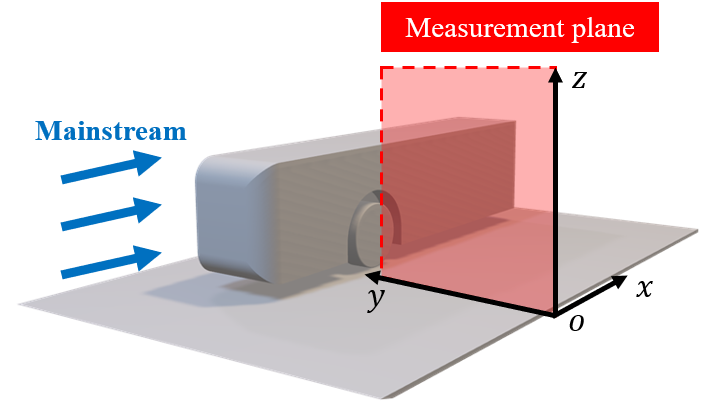
\includegraphics[keepaspectratio, width=70mm]{../images/ImageofVehicleModel.png}
  \caption{Delta wing model}
\end{figure}

\newpage
\subsection{計測結果}
Fig.6 に三角翼の計測結果と同様に 2mm 間隔の格子点上に
速度ベクトルを再配置した時間平均の結果を示す.
計測結果をみると,タイヤモデルと地面板の接触部および,
タイヤモデルの中心部に強い負の渦度が現れていることがわかる.
これらは,先行研究による数値シミュレーションおよび計測結果においても確認されており,
本手法の有効性を確認することができた.
また,本手法を用いて時刻変動のある流れ場を計測できることが確認できた.

\begin{figure}[htbp]
  \centering
  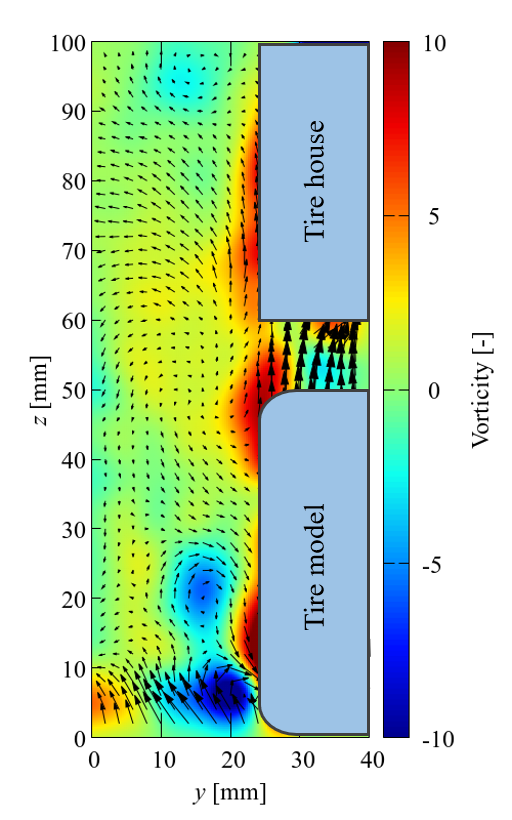
\includegraphics[keepaspectratio, width=50mm]{../images/VehicleModel_Vorticity_x=0.png}
  \caption{Wake flow of Vehicle model ($x=0$ mm)}
\end{figure}

\section{12月の予定}
\begin{itemize}
  \item 数値解析による性能評価
  \item 車両モデルの計測
  \item 修士論文の執筆
\end{itemize}

\end{document}